%# -*- coding: utf-8-unix -*-
%%==================================================
%% chapter06.tex for SJTU Master Thesis
%%==================================================

%\bibliographystyle{sjtu2}%[此处用于每章都生产参考文献]
\chapter{多模态深度学习算法}
\label{chap:chap6}

\section{多模态深度学习介绍}
	随着近些年个人计算机计算能力的显著提高,Hinton提出的深度学习也越来越受到机器学习研究者的青睐。譬如在图像和文本领域,深度学习在图像识别和文本分类等任务中都表现的令人满意。然而随着图像和文本这两个模态的信息伴随彼此而一起出现的情况与日俱增(譬如微博的图片和文本),如何利用图像和文本之间的匹配关系,挖掘出他们的共有信息成为了多模态深度学习的目标。部分已有研究(需要加注释,引用)对图像和文本的多模态深度学习已经有了比单一模态的深度学习显著优秀的结果。因此,本课题就是在利用多模态的信息来进一步提升情绪识别的效果。本文利用EEG数据和眼动仪数据作为两个模态的输入,尝试寻找两者的匹配关系,并构建共有特征表达,虽然EEG数据和眼动仪数据两者不但在量级还是特征维度上的差别都十分巨大,但是我们仍旧达到比单一使用任意一个模态进行深度学习更好的效果。
	
\section{深度自编码器}{
	本论文所使用的算法模型是基于深度自编码器的,具体的实现将在下一节中详细说明。本节目的是阐述深度自编码器的原理。
	
	根据定义,深度自编码器是由两个对称的深度置信网络组合而成。一般情况下,会有四到六层的编码层,紧跟着的是同样层数的解码层,并且编码和解码对应的每层结构都完全相同。每一层都可以认为是受限波尔兹曼机(Restricted Boltzmann Machines,简称为RBM)。编码层和解码层交汇之处就是深度自编码器学习到的的特征向量。
	
	
	在编码阶段,举例来说,譬如我们的输入数据是310维的,那么通常来讲,深度自编码器的第一层应该有略多于输入层元素个数的维度,譬如350维,这看上去有些让人困惑,因为我们都知道创建比输入维度更多的参数容易造成过拟合。但是实际上,拓展出更多的参数就相当于表示了更多输入数据的特征,只有这样才能实现最终的解码过程,这是由于sigmoid函数的表达能力决定的。一旦sigmoid函数进入饱和区,那么就会丢失很多信息,让深度自编码器的第一层有更多参数是为了补偿sigmoid函数这方面的不足。而在第一层之后,在编码的阶段里,维度应该逐层指数递减,直到最后一层,此时不进行任何分类,而只是一个RBM的隐层。我们建立好编码网络,然后在后面加上解码网络。
	
	在解码阶段,输入就是编码阶段的最后一层,这一层也就代表了编码之后的信息。正如前面所说,解码网络与编码网络对称,它的训练过程就是学习如何用编码之后的信息来重建原始输入。初始化的时候并不能随机初始化,而我们应该设置所有参数等同于编码网络对应的部分(连接权矩阵需要转置)。整个网络是利用反向传播算法来进行训练的,每次对比解码网络重建出来的值和原始输入的差,利用损失函数来计算梯度,最后更新。
	
	在利用反向传播算法进行训练的阶段,学习率应该设置的很小,有建议[参考文献http://deeplearning4j.org/deepautoencoder.html]说对于二进制数据,学习率应该设为$1 * 10^{-3}$,而对于连续数据,学习率应该设为$1 * 10^{-6}$。
	
	深度自编码器已经在多个领域有实际应用。
	\begin{itemize}
	\item 图像搜索,可以将较大的二维图像特征向量,譬如上千维的像素编码成到长度为几十的特征向量。加速搜索,返回准确结果。
	\item 数据压缩,如语意哈希(Semantic Hashing)。这是一种为文件寻找一种二进制编码的方法,使得相似度高的文件对应的编码海明(hamming)距离小,相似度低的文件对应的编码海明(hamming)距离大。可以加速文件搜索等。
	\item 主题模型和信息检索。深度自编码器可以用于自然语言处理里面的主题模型或者类似的利用统计学来在一系列文档里面建立主题的算法。具体来讲,每个文档都被转化为bag-of-word模型,也就是词频统计的特征向量,然后把词频归一化,所以每个元素都可以被认为是一个词在文档中出现的频率。接着把这个特征向量输入进由多层RBM组成的深度置信网络,并且设定网络的最后一层只有比较少的元素,譬如10个。最后,把这一层的特征作为新的特征向量,每个特征向量与一篇文档一一对应。这样每个文档可以与任何一个其他文档计算距离,距离由新的特征向量所定义。相似的文档距离近,如此一来,特征向量相似的文档应该具有类似的主题。这就是主题模型的工作原理。
	\end{itemize}
}
\section{算法模型}
	我们的目的是设计合适的网络能够接受两个模态的输入,而输出两个模态的共有特征。自然的,我们选用深度神经网络(Deep Neural Network,简称DNN)作为基本框架。不过传统的DNN都是针对单模态的,于是,我们构建了以RBM为基本单位的,多层次的多模态DNN。它可以接受两个模态的输入,并进行编码和解码过程,最终解码过后可以得到重建后的两个模态的特征。此时我们对重建后的特征和输入特征进行对比并且校正,多次迭代DNN网络就可以得到合适的网络参数,并且可以提取出网络中任意层次的共有特征表达。
	\subsection{RBM介绍}
	如果要进行深度学习的研究,那么必须要理解RBM的相关背景。\\
	\par
	\centerline{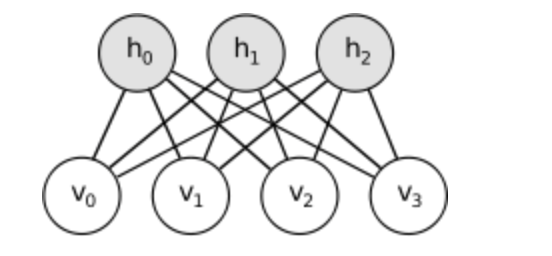
\includegraphics[width=4.5in]{figure/rbm.png}} %要居中就用centerline,这里的图片和tex 文件在一个目录下
	\centerline{图6-1}

	这是RBM的基本模型,其中v代表显层(visual), h代表隐层(hidden)。每个RBM都由一个显层和一个隐层组成,显层和隐层都可以有大于等于一的任意多个维度。而显层之间的所有单元均不相连,隐层之间的所有单元也全不相连。而两层之间的单元全相连。值得一提的是,如果所有单元保持全相连,那么这个模型就是波尔兹曼机(Boltzmann Machine),由于计算复杂度等原因,深度学习研究者通常使用RBM来构建深度网络。
	RBM是一个基于能量的模型(Energy-Based model),众所周知,一个基于能量的概率模型的概率分布由它独有的能量函数定义。对于常用的伯努利RBM来说,它的能量函数如下:
	\begin{equation}
	\begin{cases}
	E(s) = -\sum\limits_{i=1}^{n-1}\sum\limits_{j = i + 1}^{n} w_{ij}s_is_j - \sum\limits_{i=1}^n \theta_i s_i \\
	p(x) = \frac{e^{-E(x)}}{\sum\limits_t e^{-E(t)}}
	\end{cases}
	\end{equation}
	其中$s \in {0, 1}^n$  为n个单元的状态向量。 $w_{i, j}$ 为第i个和第j个单元之间的连接权,$\theta_i$为第i个单元的阈值。
	若网络中的神经元以任意不依赖输入值的顺序来更新,那么最终达到boltzmann,则训练完毕。
	具体更新过程如下:
	\begin{equation}
	\begin{cases}
	P(v|h) = \prod\limits_{i=1}^d P(v_i |h)\\
	P(h|v) = \prod\limits_{j=1}^q P(h_j |v)\\
	\end{cases}
	\end{equation}
	
	\begin{align}
	\Delta w = \eta(vh^T - v\prime {h\prime}^T)
	\end{align}
	然而由于伯努利RBM只允许显层和隐层的阈值在0,1之间,并且进行抽样更新的过程只能是1或者0。而我们的数据是在实数集上,虽然我们可以对数据进行针对每一维的归一化,从而让伯努利RBM变得可行,但是经过多次试验,我发现不同的归一化方法会产生各不相同的最终结果。为了解决这个这个问题,高斯RBM是一个不错的解决方法。它与伯努利RBM的区别在于更新过程和能量函数的计算。以下是它的具体计算方法:
	\begin{equation}
	E(v,h | \theta) = \sum\limits_{i=1}^{n_v}\frac{(v_i - b_i)^2}{2\sigma_i^2} - \sum\limits_{i=1}^{n_v}\sum\limits_{j=1}^{n_h} W_{i,j}h_j\frac{v_i}{\sigma_i} - \sum\limits_{j=1}^{n_h}c_jh_j
	\end{equation}
	
	\begin{equation}
	\begin{cases}
	P(v_i = v|h) = \mathcal{N}(v | b_i + \sum\limits_{j}h_jW_{ij}, \sigma^2)\\
	P(h_j = 1|v) = sigmoid(c_j + \sum\limits_i W_{ij} \frac{v_i}{\sigma_i^2})
	\end{cases}
	\end{equation}
	
	在根据隐层更新显层的过程中,需要根据b(显层阈值)和$\sigma_i$来确定这个神经元的高斯分布,再进行抽样。根据均值和标准差确定分布,获得抽样。
	
	在根据显层更新隐层的过程中,根据c(隐层阈值) 来确定伯努利分布,再进行抽样。 均值也就是$p(h_j| V)$, 根据这个值来确定分布,进行抽样。
	
	RBM的训练过程就是多次抽样和更新的过程。这也是一个马尔科夫链(Markov Chain)收敛的过程,每一步都是吉布斯采样(Gibbs Sampling)。吉布斯采样是用来构造多变量概率分布的随机样本的方法,特别常用于期望很难计算出来,而条件概率比较容易的得到的情况。
	
	N个元素的联合分布的吉布斯采样过程如下:每次分别对于一个元素采样,总共采样N次,就得到一个样本。具体算法如下:
	
	initialize $x_i$ : i = 1, 2, …, n, T samples:
	
	for t in range(1, T):\\

	\begin{equation}
	\begin{cases}
		x_1^{(t+1)} \sim p(x_1 | x_2^t, x_3^t,…, x_n^t)\\
		x_2^{(t+1)} \sim p(x_2 | x_1^({t+1)}, x_3^t,…, x_n^t)\\
		……\\
		x_j^{(t+1)} \sim p(x_j | x_1^{(t+1)},…,x_{(j-1)}^{(t+1)},x_{(j+1)}^t,…, x_n^t)\\
		……\\
		x_n^{(t+1)} \sim p(x_n | x_1^{t+1}, x_2^{t+1},…, x_{(n-1)}^{t+1})\\
	\end{cases}
	\end{equation}
	
	利用高斯RBM我们取得了比伯努利RBM更好的结果。
	\\
	\\
	然而,如果真的使用吉布斯采样的方法来训练RBM,那么整个过程需要迭代多次,变的十分缓慢。于是,这里本文应用的是对比散度(Contrasive Divergence, 简称CD)算法,它可以大大缩减整个抽样迭代的步数。
	
	CD算法由G. Hinton提出,用于求极大似然问题(Maximum-Likelihood)的近似解。它的基本思想是,我们想要得到P(v)分布的样本,而我们已有了训练样本,可以假设训练样本自然就是服从分布P(v)的。因此,我们的上述算法第一步初始化过程就不再是随机初始化,而是从任意一个训练样本开始。
	
	因此,CD算法的具体步骤是:从样本集合也就是训练集合任意一个样本$v^0$开始,经过k次吉布斯采样。即对于第t步采样,具体算法如下:
	\begin{equation}
	h^{t-1} \sim P(h|v^{t-1})
	v^t \sim P(v|h^{t-1})
	\end{equation}
	不断迭代我们就得到了样本$v^k$。有了采样出来的$v^k$,我们把它认为是近似的期望,所以就可以计算出梯度的近似值,并且根据其进行RBM的更新了。
	值得注意的是,在实际应用中,往往t等于1,也就是只采样一次就够了,这也就是为什么CD算法会远远快于吉布斯采样算法。
	CD算法的伪代码请见算法6-1。\\ \\
	\textbf{算法6-1(CDK算法)}\\
	输入:k(步数), S(训练集合),W(权值矩阵), a(可见层单元阈值), b(隐层单元阈值)\\
	输出:$\Delta W, \Delta a, \Delta b$\\
	第一步:初始化三个输出参数均为0.\\
	第二步:For All v $\in$ S DO:
	
		\qquad $v^0 := v;$
		
		\qquad For t in range (1, k) DO:
		
			\qquad \qquad $h^t= sampleHiddenGivenVisual (v^t, W, a, b)$
			
			\qquad \qquad $v^{t+1}= sampleVisualGivenHidden(h_t, W, a, b)$
			
		\qquad For i in range(1, $n_h$):
		
		\qquad \qquad For j in range(1, $n_v$):
		
		\qquad \qquad $\Delta W_{i, j} += [P(h_i = 1|v^0)v_j^0 - P(h_i = 1|v^k)v_j^k]$
		
		\qquad \qquad $\Delta a_j += [v_j^0 - v_j^k]$
		
		\qquad \qquad $\Delta b_i += [P(h_i = 1| v^0) - P(h_i = 1|v^k)]$
		
	而有了CD算法以后,我们就可以顺利总结出深度网络的基本单元RBM的整个算法了,这是整个深度网络的基础,请见算法6-2。\\ \\ \\ \\ 
	\textbf{算法6-2 RBM训练算法}\\
	第一步:初始化(initialization)
	
		\qquad 给定训练集合S。q
		
		\qquad 给定训练周期J,学习速率l,以及CD-k算法的参数k。
		
		\qquad 给定隐层的单元数目$n_h$,因为可见层单元数目由特征维数决定。
		
		\qquad 初始化a, b, W。三个参数矩阵或向量。\\
	第二步:训练
		
		\qquad For iter in range(1, j) DO
		
		\qquad \qquad 调用CD-k算法,生成$\Delta W, \Delta a, \Delta b$
		
		\qquad \qquad 按照算法6-1来更新这三个参数直到循环结束
		
	\subsection{模型I}
		\centerline{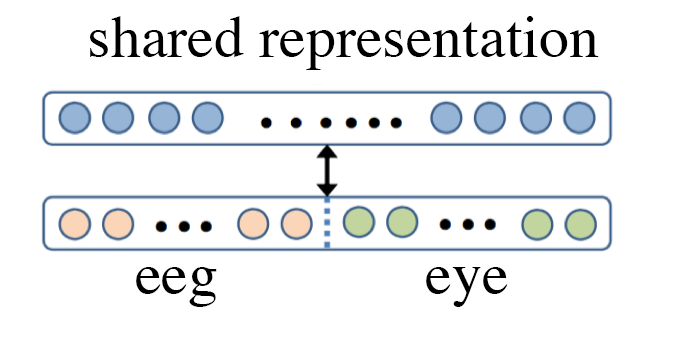
\includegraphics[width=4in]{figure/model1.png}} 
		\centerline{图6-2}
	
	如图所示,这个算法模型的功能是接受两个模态的输入,提取出两个模态的共同特征表达并输出。它的输出可以放到其他分类器,譬如SVM,神经网络等。这是一种比较直观,简单易懂的方法。那就是首先把眼动仪数据(图中eye)和脑电数据(图中eeg)直接进行拼接,两者时间窗口相同,数据也同时采集,所以样本数量相同。设眼动仪数据每个样本有n维,而脑电数据每个样本有m维,那么此时把它们拼接,得到(m + n)维的向量作为每个样本的特征。然后利用预训练之后的RBM进行特征提取,就得到了脑电数据和眼动仪数据的共同特征表达。
	
	然而,这个模型的缺点十分明显,就是这并不是一个深度的学习器,而是一个只有一层的网络,隐层和显层是线性连接的,所以这个模型很难找到眼动仪数据和脑电数据的非线性关系,并不能提取出理想的共同特征。
	
	为了解决这个问题,只能构建更深层次的网络。	
	\subsection{模型II}
		\centerline{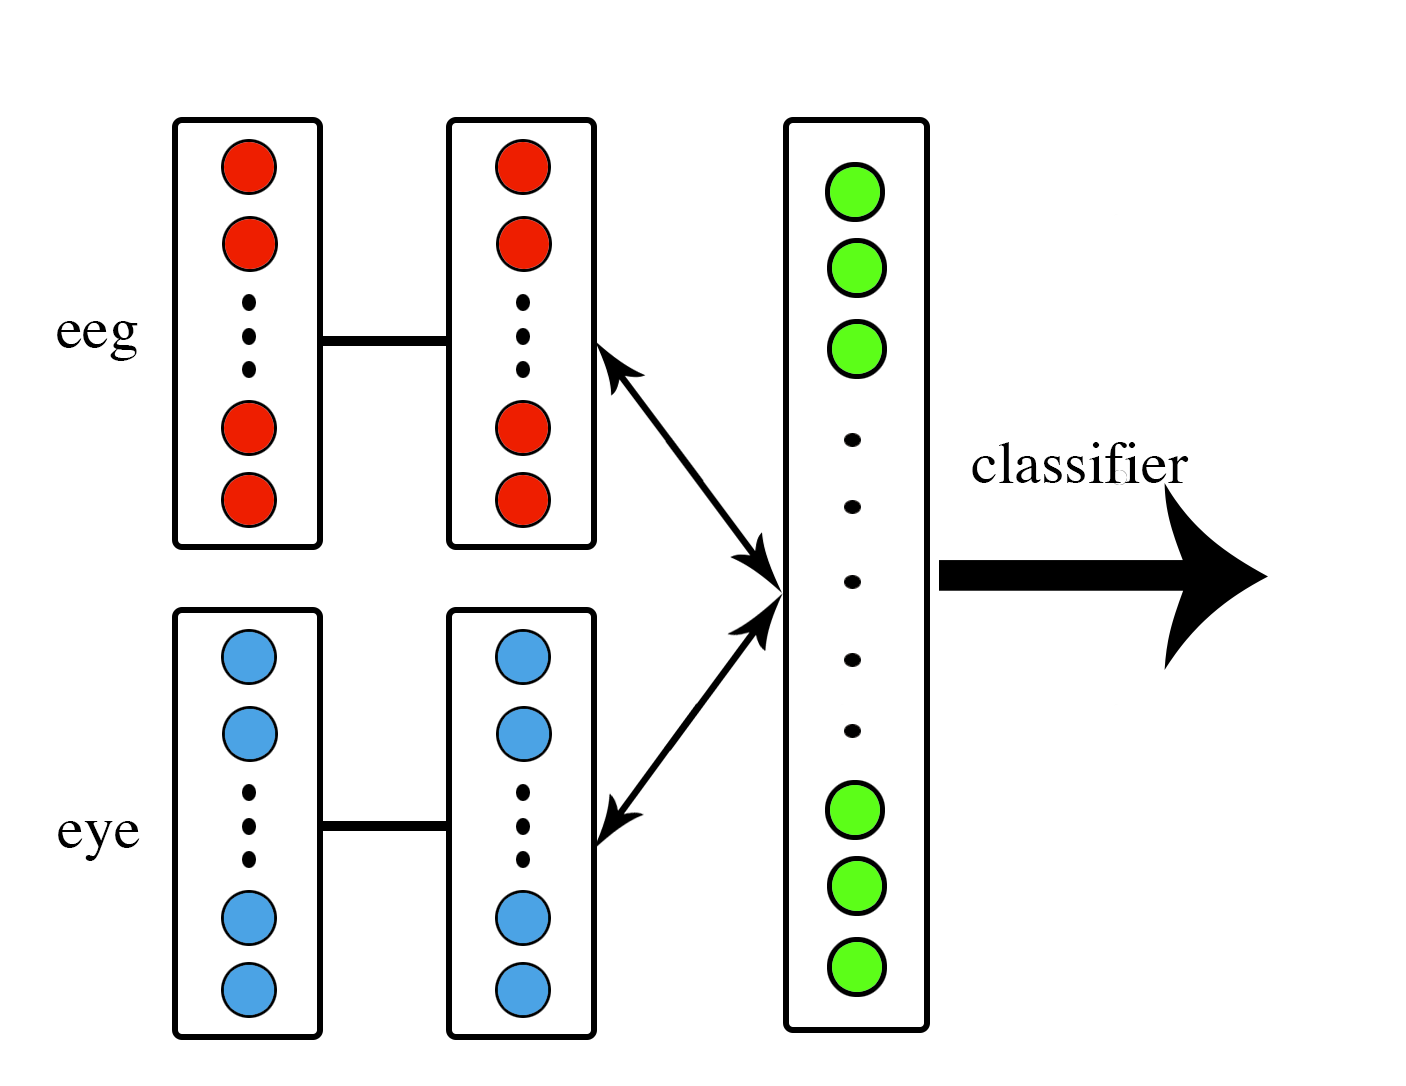
\includegraphics[width=5in]{figure/classify1.png}}
		\centerline{图6-3}
		如上图所示,此算法模型的功能与模型I类似,只是更加复杂,它可以更好的学习到两个模态的数据之间的非线性关系。首先用两个RBM分别提取眼动仪模态和脑电模态的特征,然后再将提取后的特征拼接,并再加一层网络提取共同表达的特征。这个网络一共包含三个RBM,在经过预训练和调参之后,我们获得了比模型I更好的结果。
		
		值得一提的是,模型I与模型II中每个RBM我们尝试了伯努利RBM和高斯RBM,然而在后续工作中我们发现在每个RBM的每个元素中都使用修正线性单元(Rectified Linear Unit,简写为ReLu)替代了sigmoid unit之后,便不再需要预训练,因此这个问题也就无需再考虑,因为不论是从速度还是结果来看,前者都是更优秀的。下文中将对这两个激活函数进行更详尽的对比。
	\subsection{模型III}
		\centerline{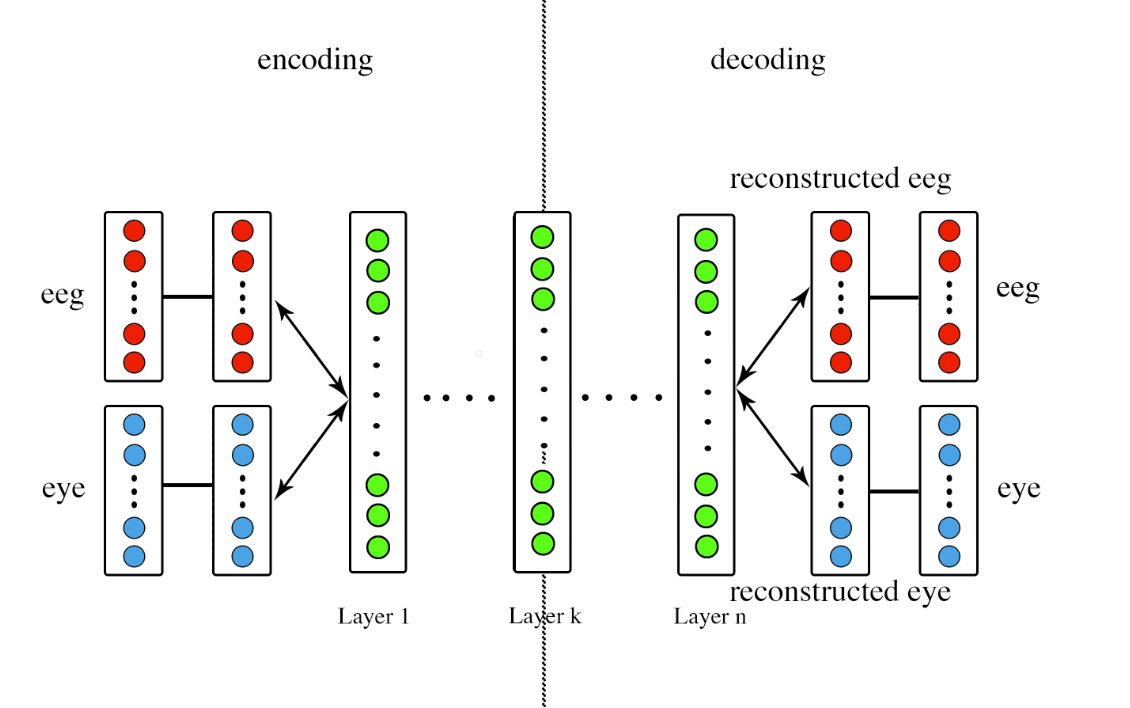
\includegraphics[width=7in]{figure/feature_learning.png}}
		\centerline{图6-4}
		
		如上图,这就是本文构建的特征提取算法模型。与前两个模型一样,它也接受两个模态的输入,并输出共同特征表达,用于后续的情绪识别任务。
		
		这个算法模型的左边是输入,右边是计算结果。我们把整个特征提取过程的一次迭代分成两个部分,左边半部分是编码过程(encoding),右边半部分是解码过程(decoding)。编码过程和解码过程应该是完全对称的,编码过程是学习更深层次特征的,解码过程是重建数据的。本模型首先分别对两个模态用RBM提取特征,然后对提取后的特征进行拼接,再加上k层网络增加深度来学习两个模态的非线性关系。图片中间的一层是编码的最后一层,也是解码的第一层。整个模型越靠中间的层,深度越深,也就代表了越抽象的特征,越靠近两边的层深度越浅,也就代表了越具体的特征。当计算到最右边一层的重建特征时,我们把整个特征向量一分为二,重新变为脑电数据和眼动仪数据两个模态,然后用输入数据和网络重建的数据进行对比,计算方差来校正整个网络的参数。 注意,即使最左边是数据输入,网络看似越靠右的层有越抽象,越深层次的特征,但是由于我们网络和更新算法的定义,编码过程里面才是越靠右的层越抽象的,而解码过程里面越靠右的层有越具体的特征,因为整个解码过程都在重建原本的特征,所以是不断变的更加具体的。
		
		然而,不像图像识别任务一样,深度网络的每个层次的特征都代表明确的意义,譬如浅层可能是直线和曲线,深层就是复杂的轮廓。趋势是越浅层的越局部越具体,越深层的越广泛越抽象。脑电和眼电数据的深度学习网络里,每个层次的数据并没有明确的意义。为了找出哪个层次的共同特征表达最适用于我们的情绪分类任务,我把从第一层到第n层的共同特征全部提取出来,并进行试验,得到了最终的结果。示意图见下方:
		\centerline{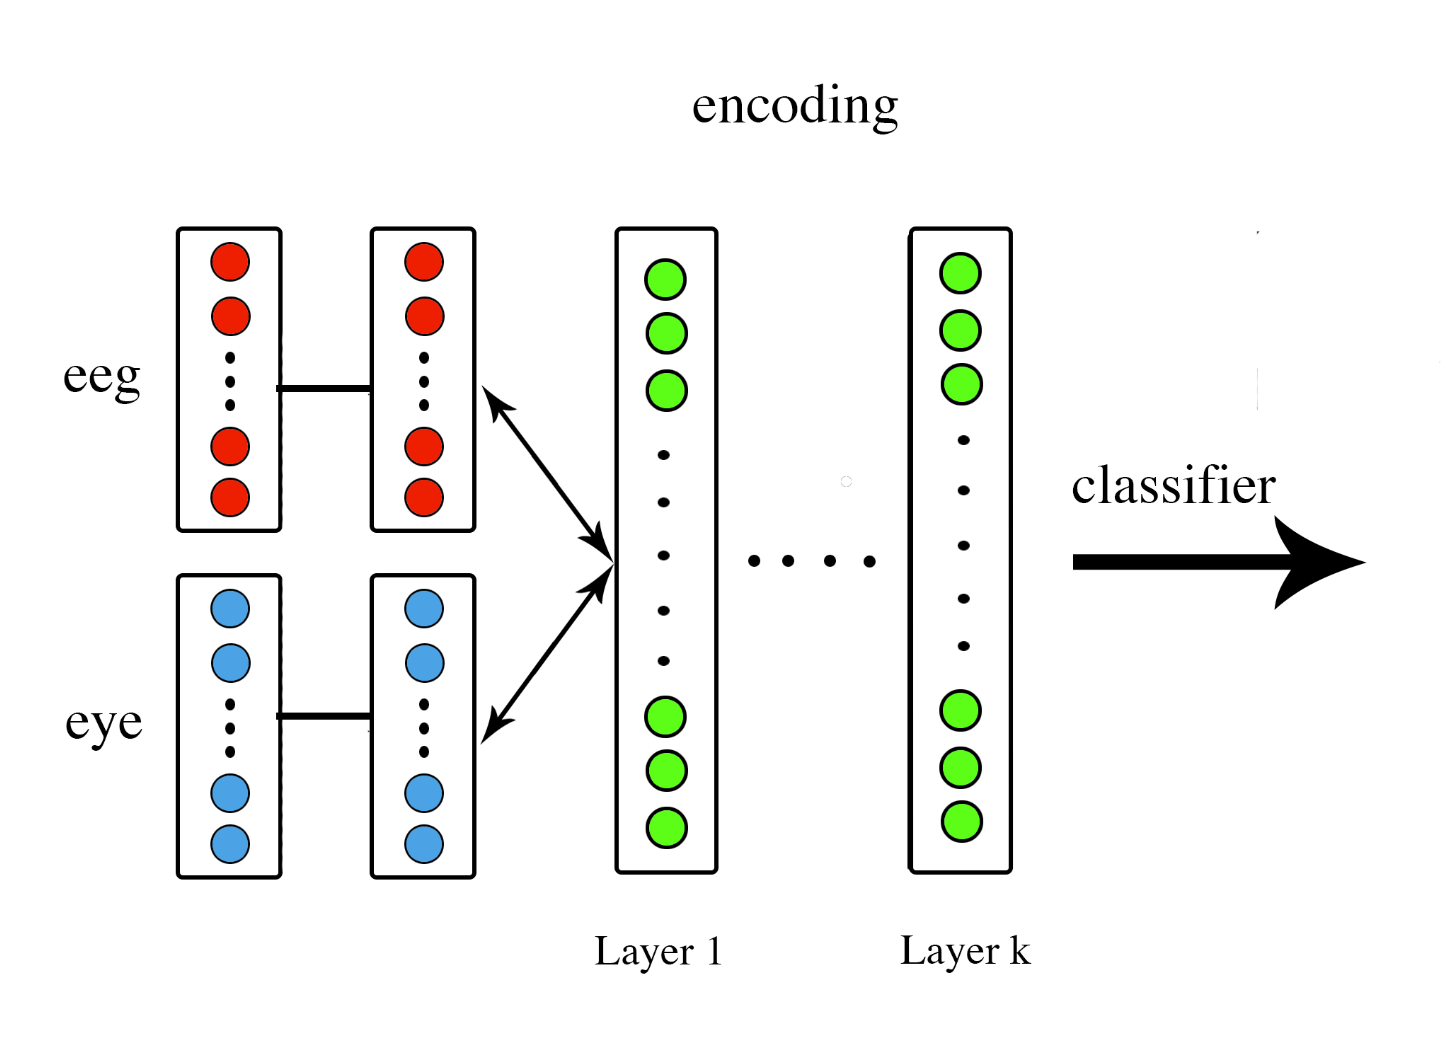
\includegraphics[width=5in]{figure/classifyk.png}}
		\centerline{图6-5}
		\centerline{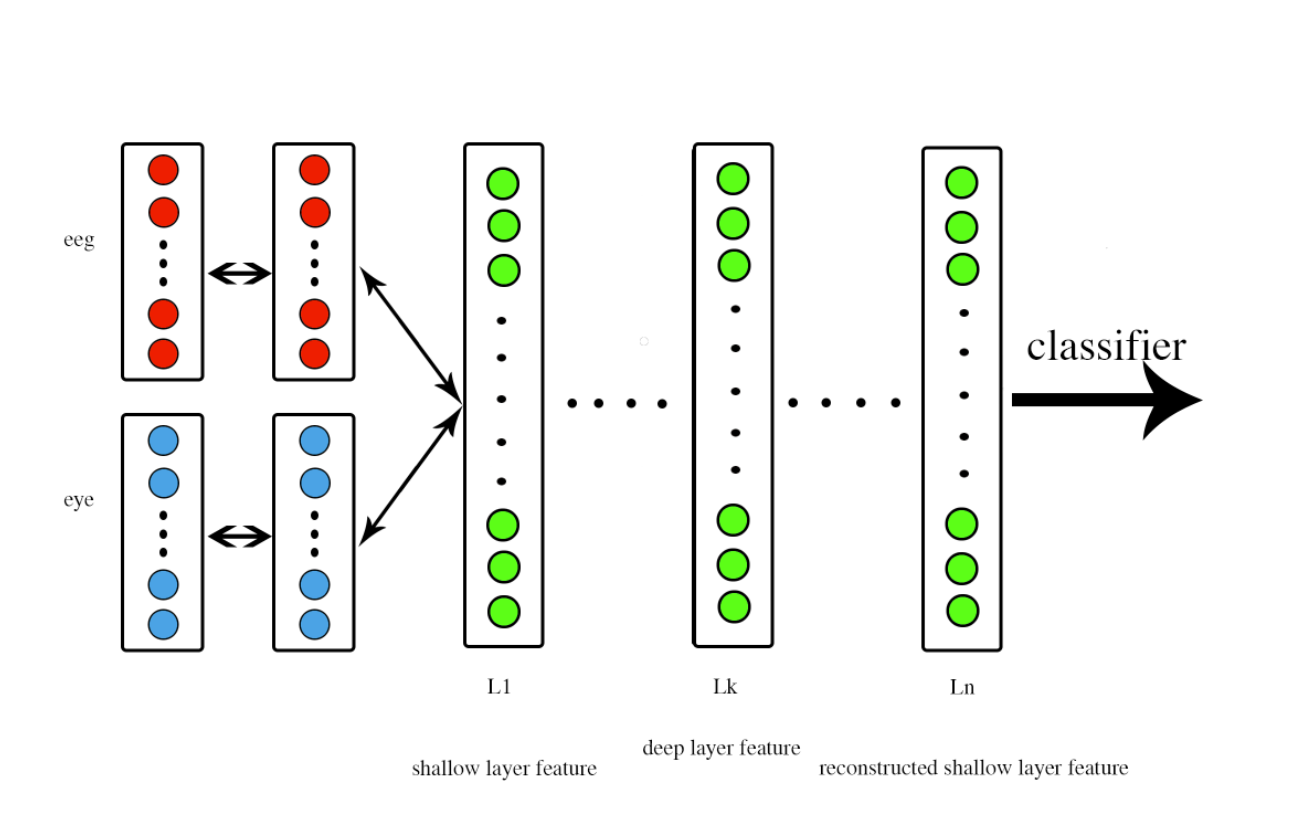
\includegraphics[width=5in]{figure/classifyn.png}}
		\centerline{图6-6}
		
		\centerline{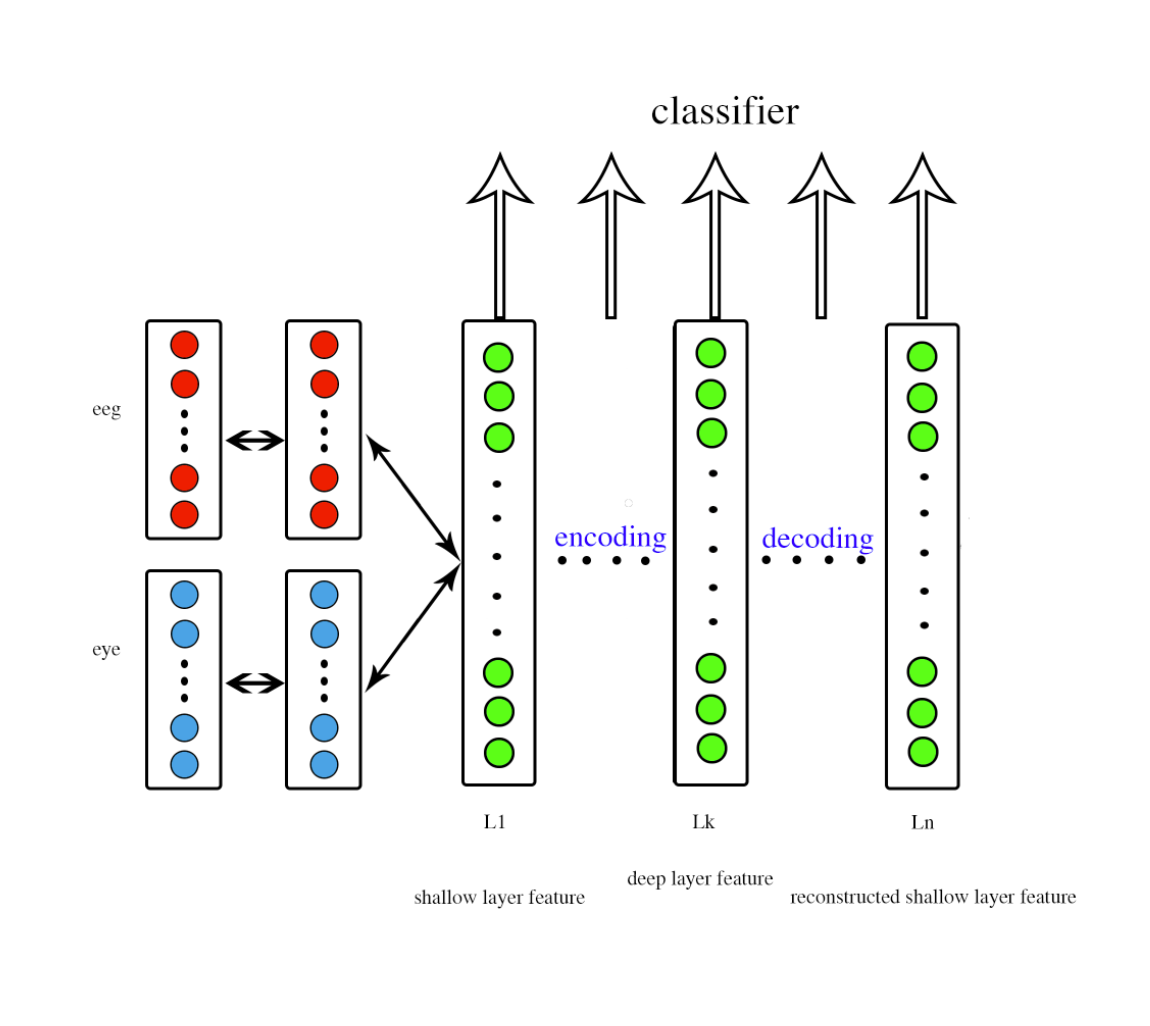
\includegraphics[width=5in]{figure/classify_all.png}}
		\centerline{图6-7}
		
	\subsection{激励函数的改进}
		
		一直以来,sigmoid函数由于其独特的性质,被广泛的用于神经网络中作为神经元的激励函数。然而最近研究者发现,修正线性单元有成为更加优秀的激励函数的潜力。本论文从理论和实验结果两方面均对这两族函数进行了对比。与线性修正单元近似的一个函数是softplus,两者的定义如下。
		\begin{equation}
		SoftPLus: f(x) = \quad ln(1 + e^x)\\
		ReLu:  f(x) = \quad max(x, 0)
		\end{equation}
		首先,sigmoid函数一直以来对机器学习的贡献巨大,这是因为它是非线性的激励函数。如果我们不用非线性激励函数,而是直接用$f(x) = x$作为我们的激励函数,那么显而易见,网络的每一层输入都是上一层输出的线性组合,这样一来无论网络有多深,每层有多少个神经元,最终输出总是输入的线性组合,隐藏层就失去了意义,神经网络模型就退化成了最简单的感知机模型。而一旦我们引入sigmoid这样的非线性激励函数,那么每一层就不再是上一层的简单线性组合,而是可以逼近任何函数。并且,sigmoid函数的输出永远在0和1之间,范围确定,很适合作为下一层的输入,哪怕网络十分深,也不会面临指数爆炸等问题。这是神经网络算法的基础。
		
		线性修正单元在2011年被首次提出可以作为一种非线性的激励函数使用在有监督的深度神经网络中,并且它的应用可以避免无监督的预训练。[注释1]线性修正单元不但具备sigmoid函数的很多优点,还具备更加优秀的性质,可以补偿sigmoid不尽如人意的地方。研究者之所以对线性修正单元投入越来越多的精力,主要有以下几点原因:
		\begin{enumerate}
		\item 采用sigmoid函数的时候,算激活函数时是指数运算,计算量大。
		\item 反向传播求误差梯度时,求导涉及除法,计算量相对大,而采用Relu激活函数,整个过程的计算量节省很多。
		\item 对于深层网络,sigmoid函数反向传播时,很容易就会出现梯度消失(vanishing gradient)的情况,因为每一层都可能会小一个数量级。
		\item Relu会使一部分神经元的输出为0,这样就造成了网络的稀疏性,并且减少了参数的相互依存关系,避免了过拟合问题(over-fitting)的发生。
		\item Relu函数没有上界,那么前期梯度值可以很大,如此一来训练前期权值可以较大幅度的调整。通过这样来起到加速的效果。
		\item 对于我们的数据来说,如果我们想用sigmoid函数作为激励函数,那么必须要将数据归一化到[0,1]范围内,否则的话我们是在函数的饱和区内,而不在函数剧烈变化的非饱和区内,相当于全部维度都是冗余信息,也就是传播的过程中丢失了大量的信息[Glorot, X., Bordes, A., and Bengio, Y. (2011b). Deep sparse rectifier neural networks. In JMLR CP: Proceedings of the Fourteenth International Conference on Artificial Intelligence and Statistics (AISTATS 2011). 130, 297]。而不同归一化结果会产生不同结果,这个冗余的步骤会对结果带来不好的影响。如果用ReLU就解决了这个问题,不再需要进行归一化。
		\item 实验证明,ReLu激活函数可以避免了预训练的流程,节省了训练网络所需要的时间和步骤。
		
		\end{enumerate}
		
		另外,线性修正单元还有一些变种,适用于不同的情况。譬如:
		\begin{itemize}
			\item{
				噪声线性修正单元(Noisy ReLUs)
				
				当线性修正单元被拓展,允许有高斯噪声加入其中后,我们就称它为噪声线性修正单元。 它作为激励函数在计算机视觉领域的应用较为成功。它的函数式如下:
				\begin{align}
				\begin{cases}
					f(x) = max(0, x + Y)\\
					Y \sim \mathcal{N}(0, \sigma (x))
				\end{cases}
				\end{align}
			}
			\\
			\item{
				渗透线性修正单元(Leaky ReLUs)
				
				当所属单元没有被激活的时候,渗透线性修正单元允许产生非零的梯度,它的函数式如下:
				\begin{align}
				f(x) = 
				\begin{cases}
					x & if x > 0 \\
					0.01x & otherwise
				\end{cases}
				\end{align}			
			}
			\item{
				含参线性修正单元(Parametric ReLU)
				
				含参线性修正单元在渗透线性修正单元之上更进一步,它含有接受一个参数a,就像其他的连接权和阈值一样,a也是由神经网络逐渐学习而不断更新的。含参线性修正单元函数式如下:
				\begin{align}
				f(x) = 
				\begin{cases}
					x & if x > 0 \\
					ax & otherwise
				\end{cases}
				\end{align}
			}
		\end{itemize}
		
		
		
		综上所述,线性修正单元作为一种与sigmoid函数相似的函数,虽然它有潜在的问题就是在0处不可导,但是综合来说它可以在复杂的数据集上达到更好的效率和表现。
		